% !TeX spellcheck = de_DE

\chapter{Cheat Sheet}


\marginpar{Funktion}%
Nachdem das Kamerabild eingelesen worden ist, sollen die entsprechenden Objekte gefunden werden. Mit diesen Informationen soll dann der Abstand zum Objekt ermittelt werden und via serielle Schnittstelle an die Fahrplattform übertragen werden.




\section{Listing}
\begin{enumerate}[label=(\alph*)]
	\item Pixelwert wird unterdrückt (Wert = 0), da es sich nicht um das Maximum in die Gradientenrichtung $- \pi$ handelt
	\item Bildet das lokale Maximum in Gradientenrichtung $\frac{3 \pi}{4}$, Pixelwert wird nicht verändert
	\item Bildet auch das lokale Maximum in Gradientenrichtung, Pixelwert wird nicht verändert
\end{enumerate}


\section{Cite and reference and format}

Reference: \autoref{fig:hsv2} \\


Cite: \cite{xlinuxai}\\


Package: \package{TFLite Model Maker} \\

Footnote: \footnote{{https://www.tensorflow.org/lite/guide/model\_maker}}

\section{Images}

\begin{figure}[H]
	\centering
	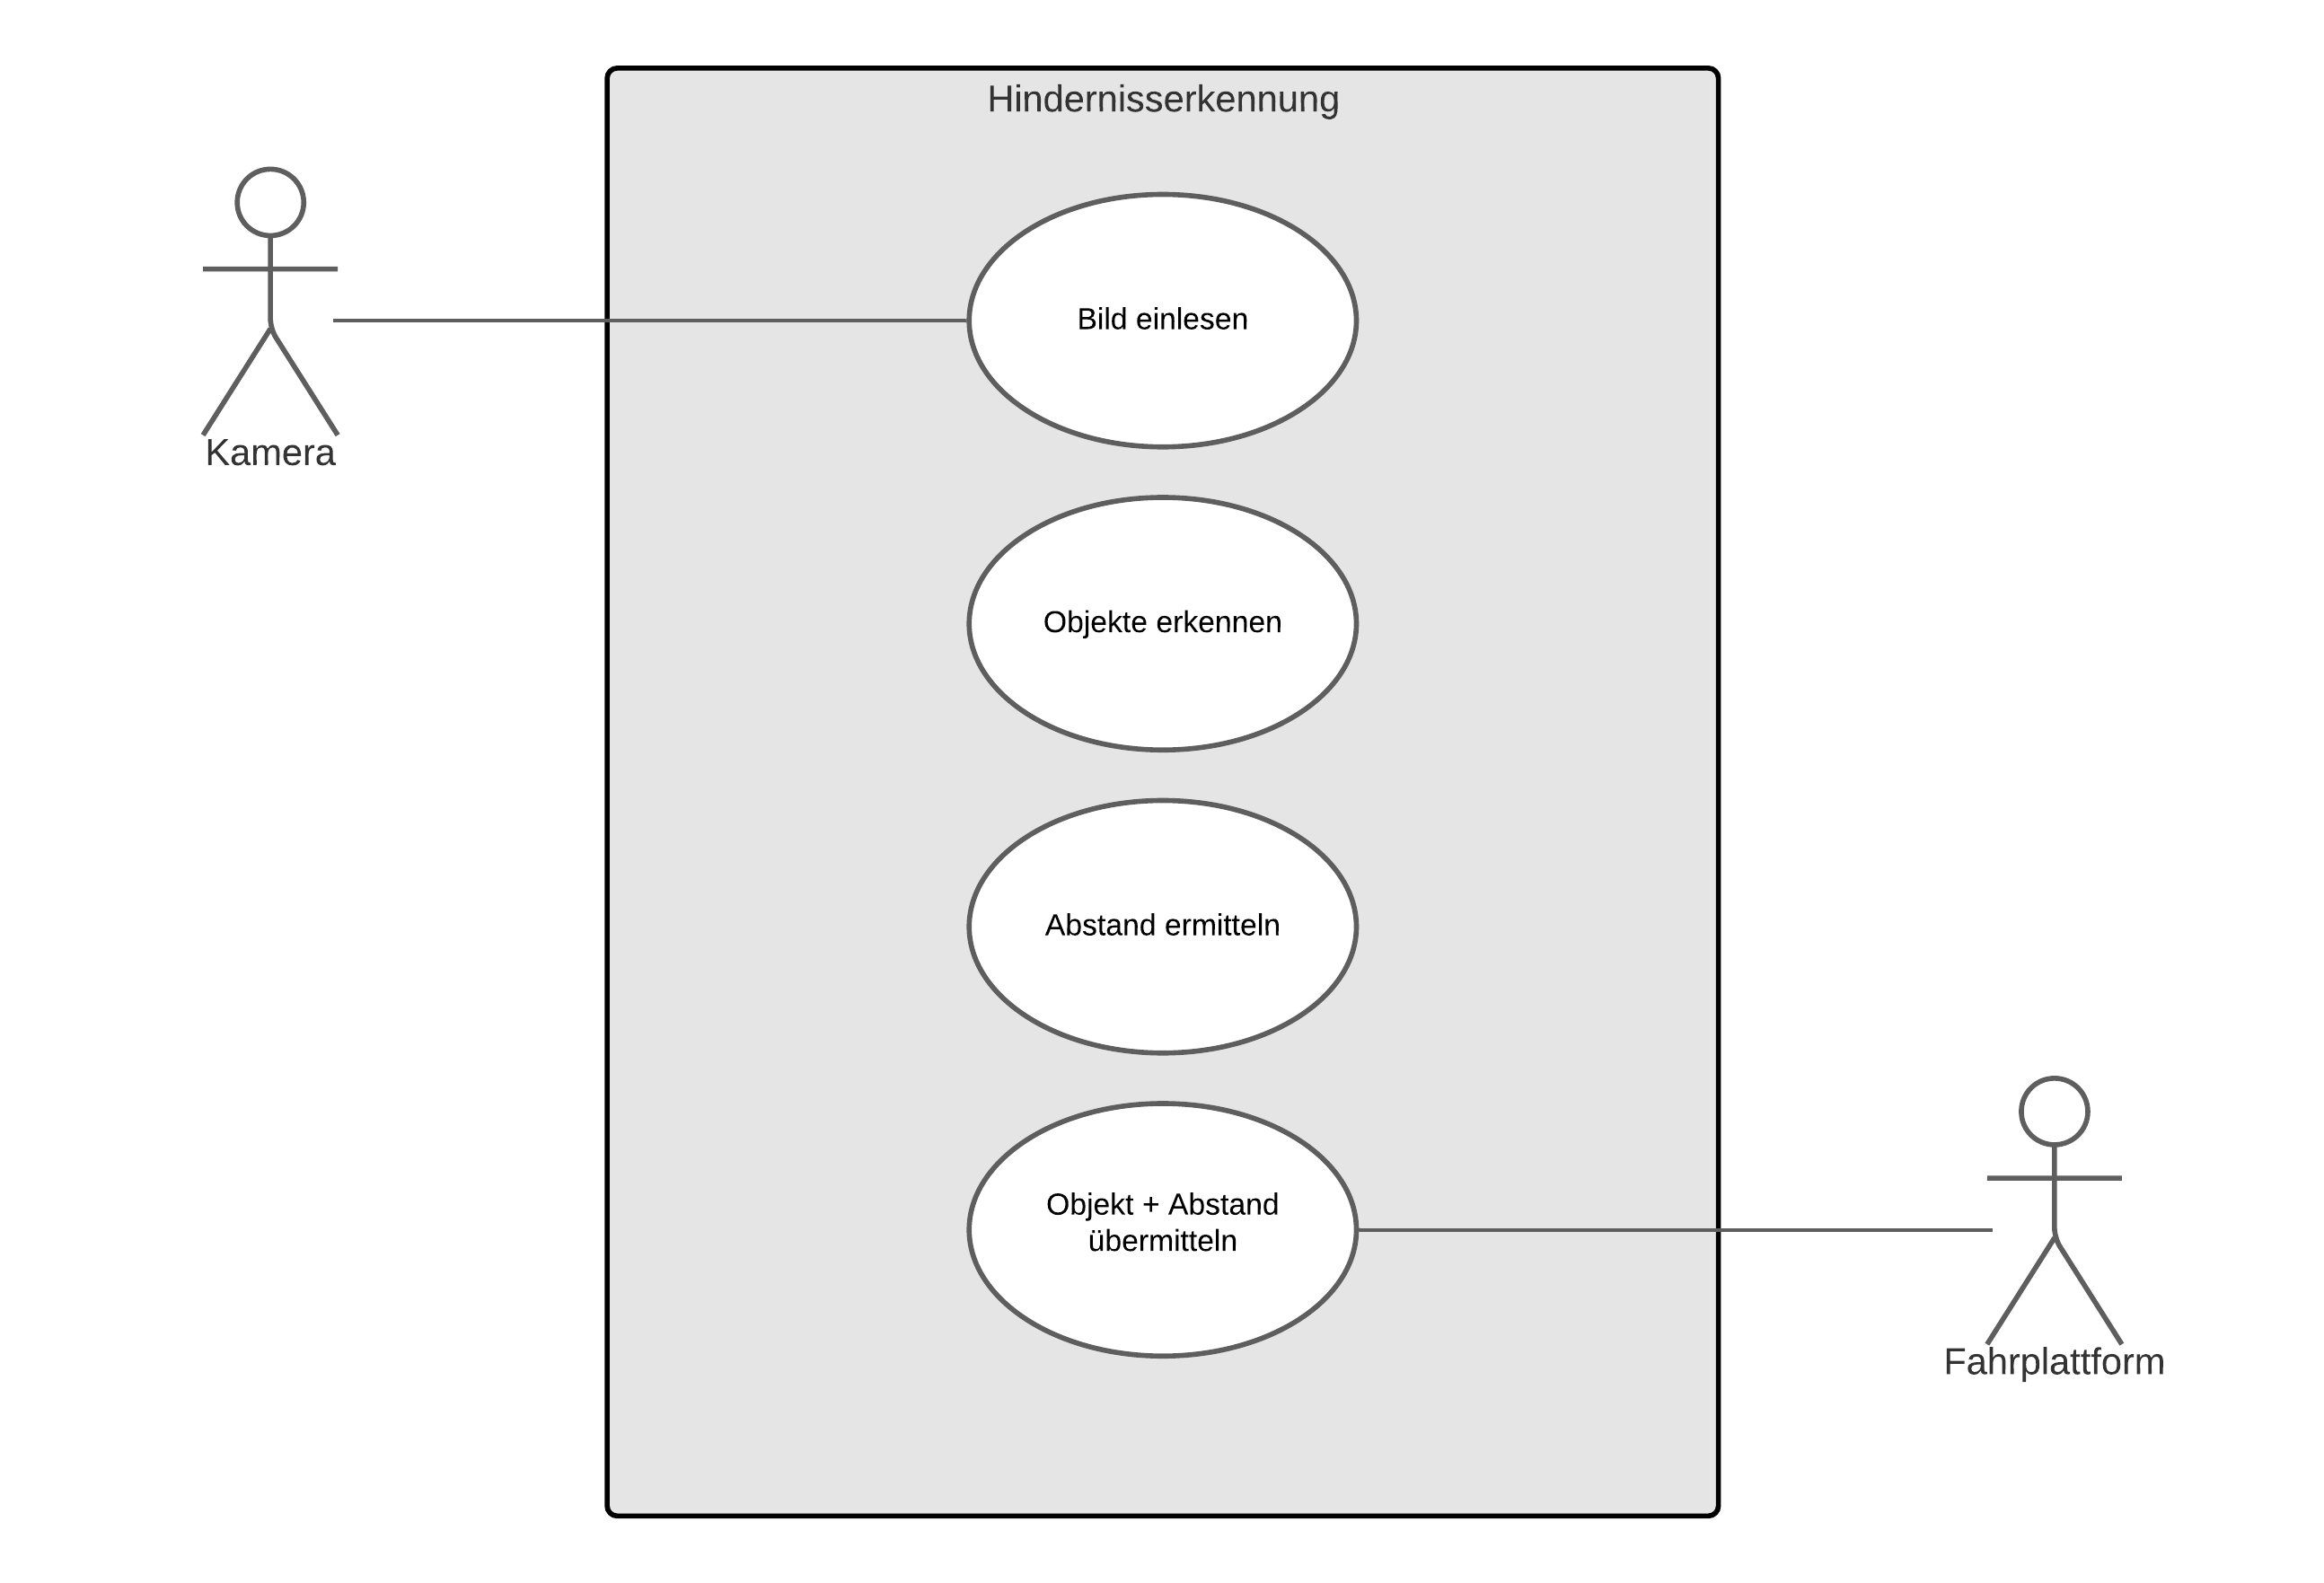
\includegraphics[width=0.35\textwidth]{chapters/cheatsheet/images/UseCaseNeu.png}
	\caption[Use Case Diagramm - Eigene Darstellung]{Use Case Diagramm}
	\label{fig:usecase1}
\end{figure}

\begin{figure}[H]
	\begin{subfigure}{0.3\textwidth}	
		\centering
		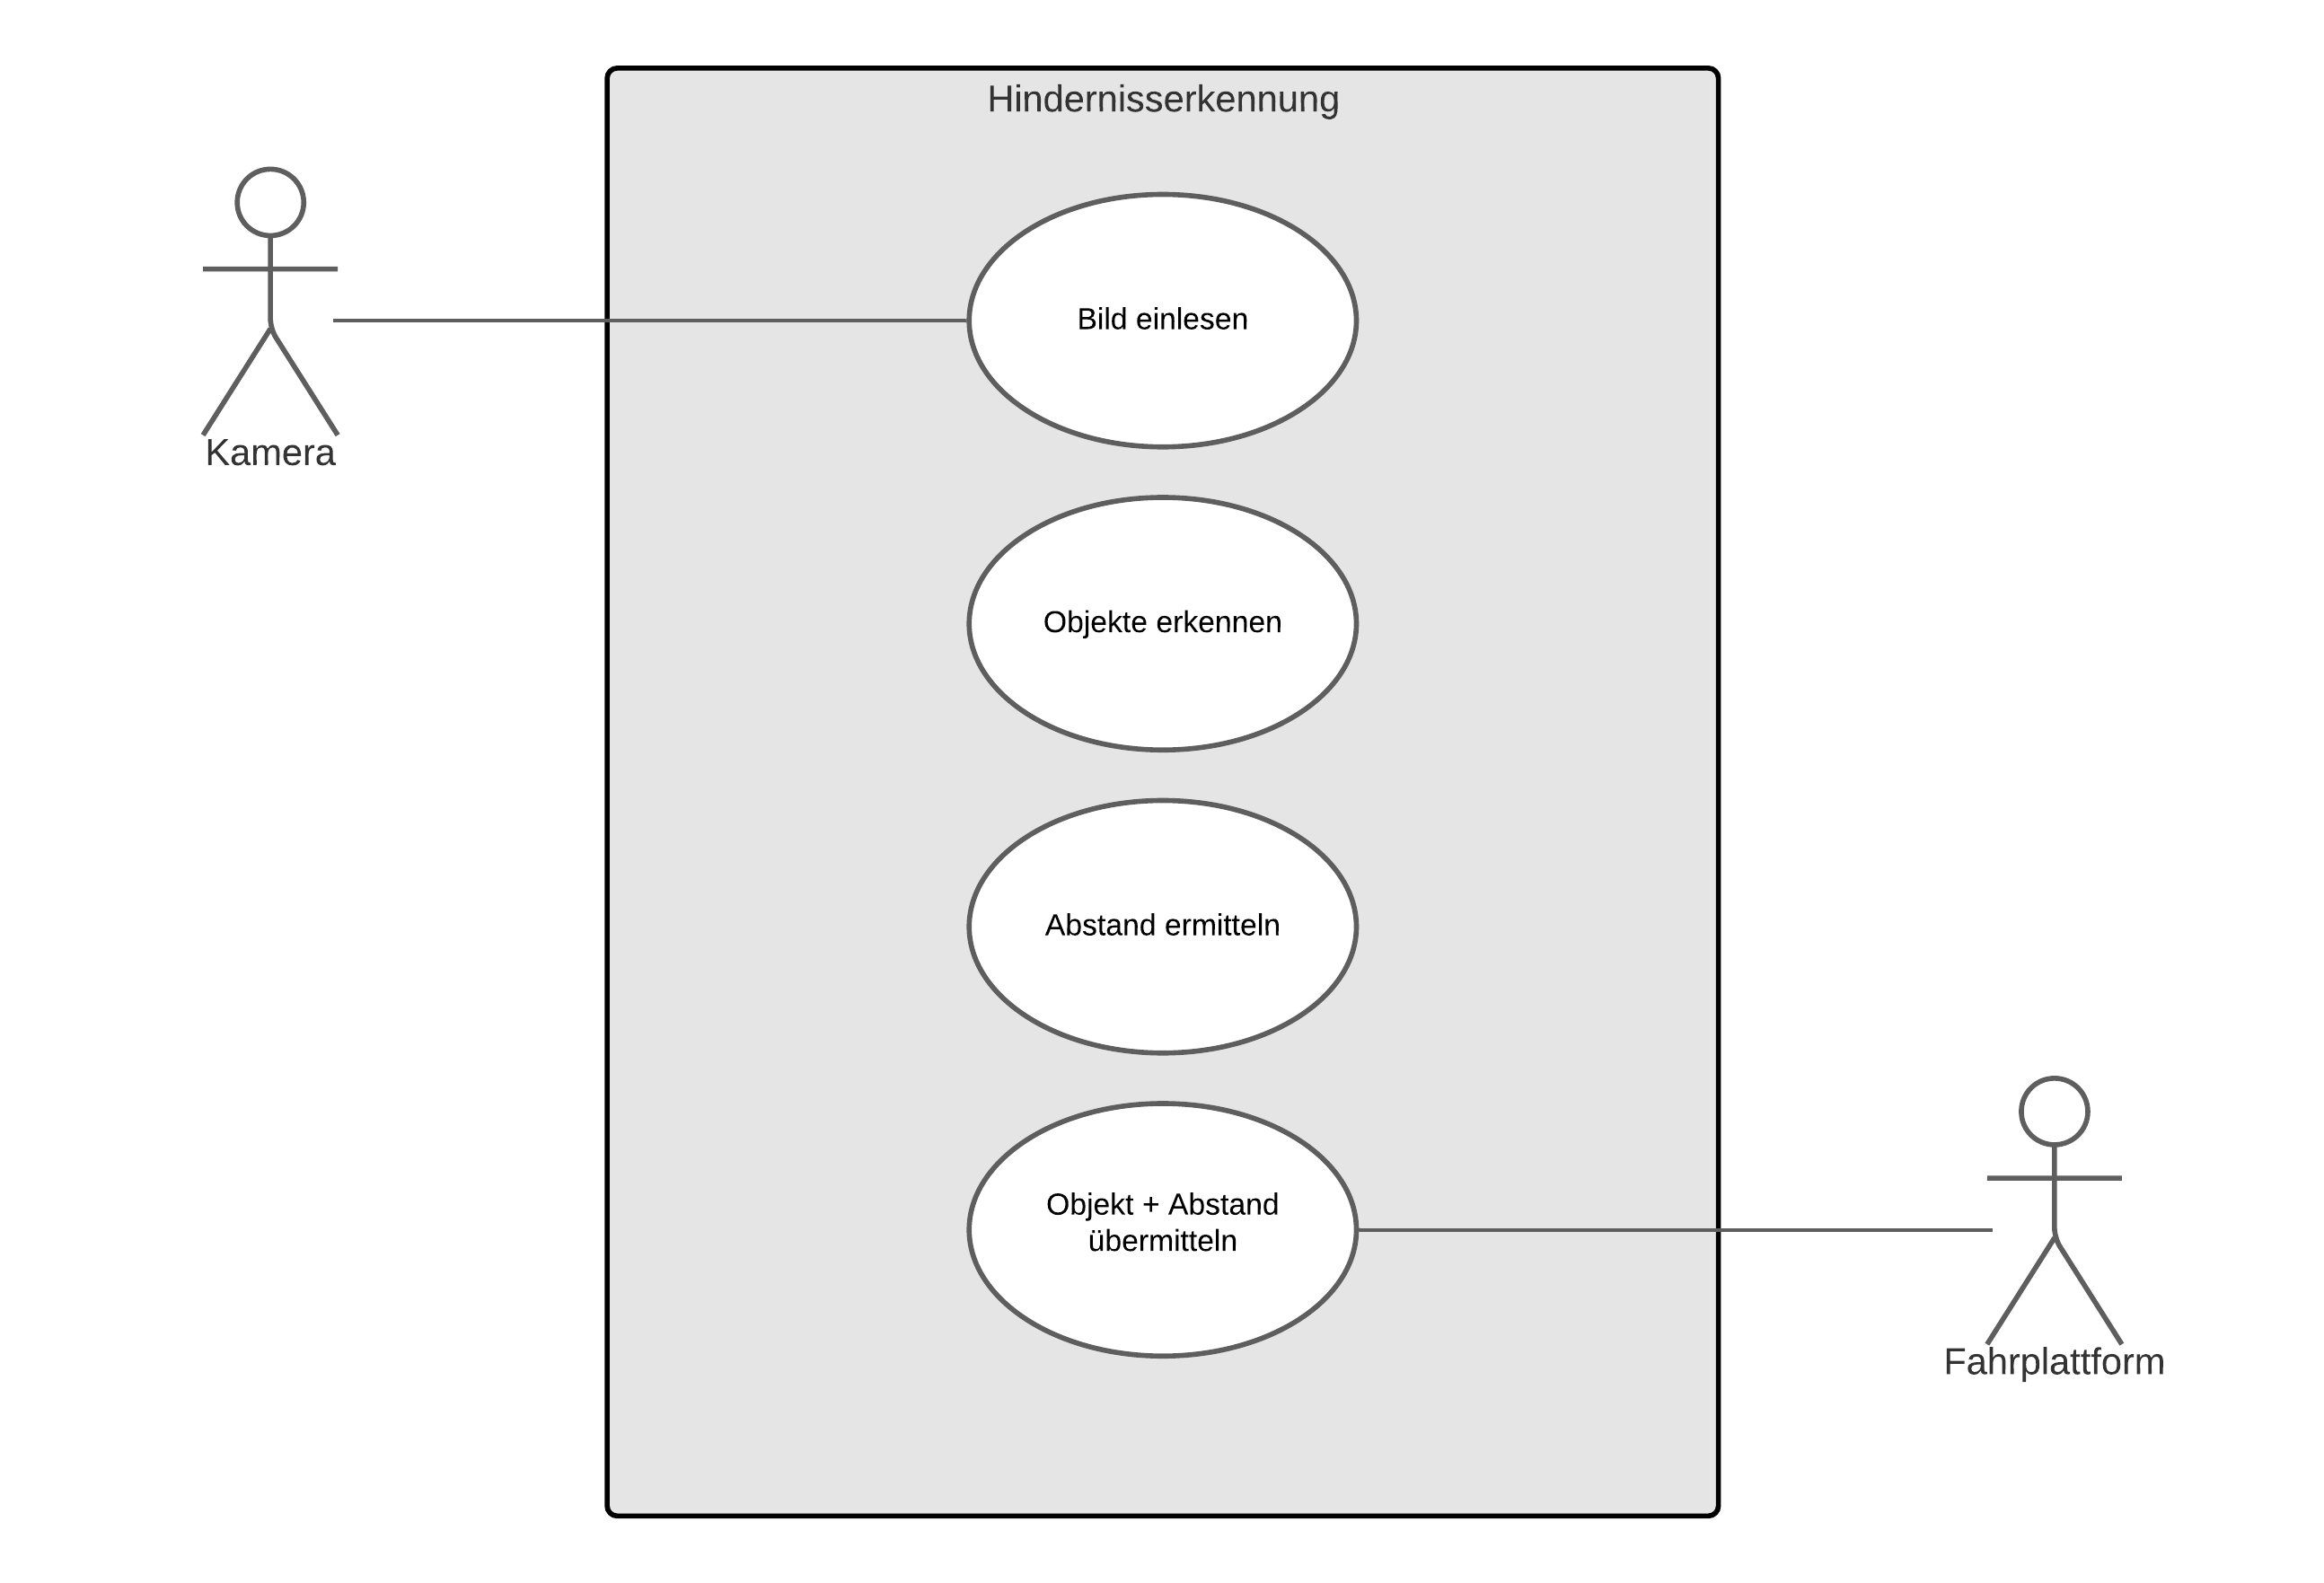
\includegraphics[width=1\textwidth]{chapters/cheatsheet/images/UseCaseNeu.png}
		\caption[HSV Farbraum 3D - Bildquelle: \cite{opencvfarbraum}]{3D \cite{opencvfarbraum}}
		\label{fig:hsv1}
	\end{subfigure}%
	\begin{subfigure}{0.7\textwidth}
		\centering
		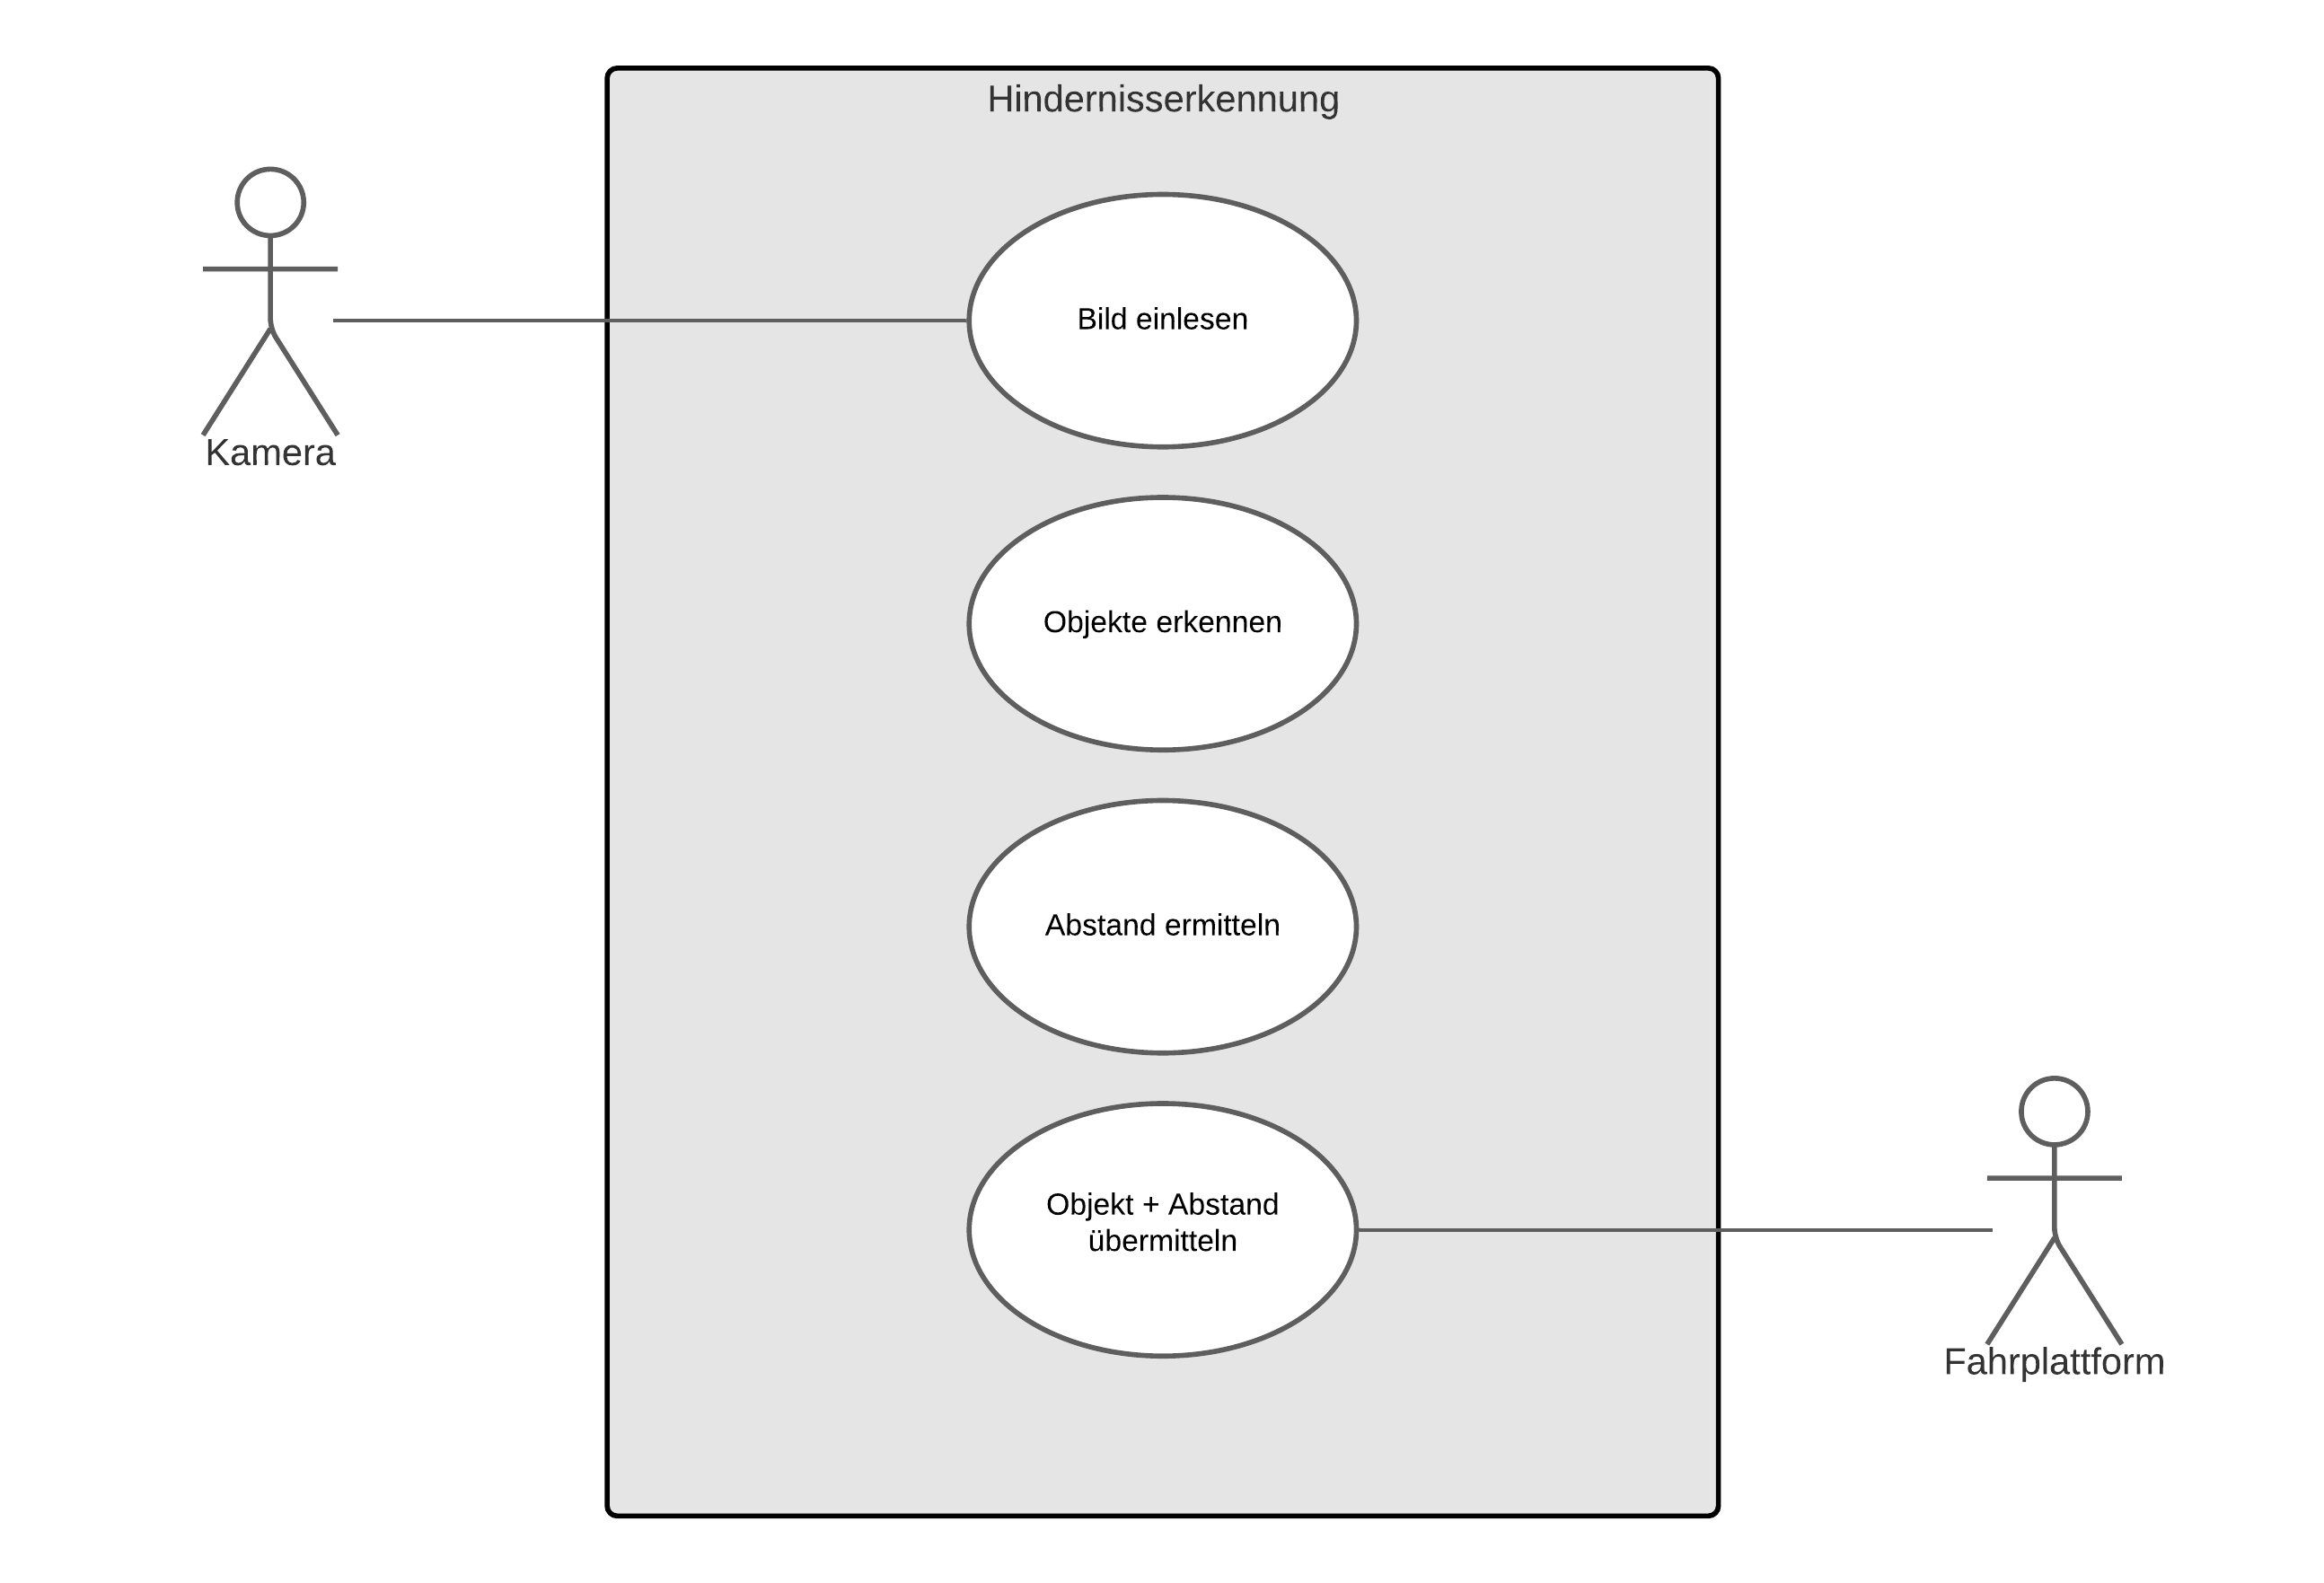
\includegraphics[width=0.8\textwidth]{chapters/cheatsheet/images/UseCaseNeu.png}
		\caption[HSV Farbraum 2D - Bildquelle: \cite{hsv1}]{2D \cite{hsv1}}
		\label{fig:hsv2}
	\end{subfigure}%
	\caption[HSV Farbraum - Bildquelle: \cite{hsv1}]{HSV Farbraum}
\end{figure}


\begin{figure}[H]
	\begin{subfigure}[t]{0.35\textwidth}	
		\centering
		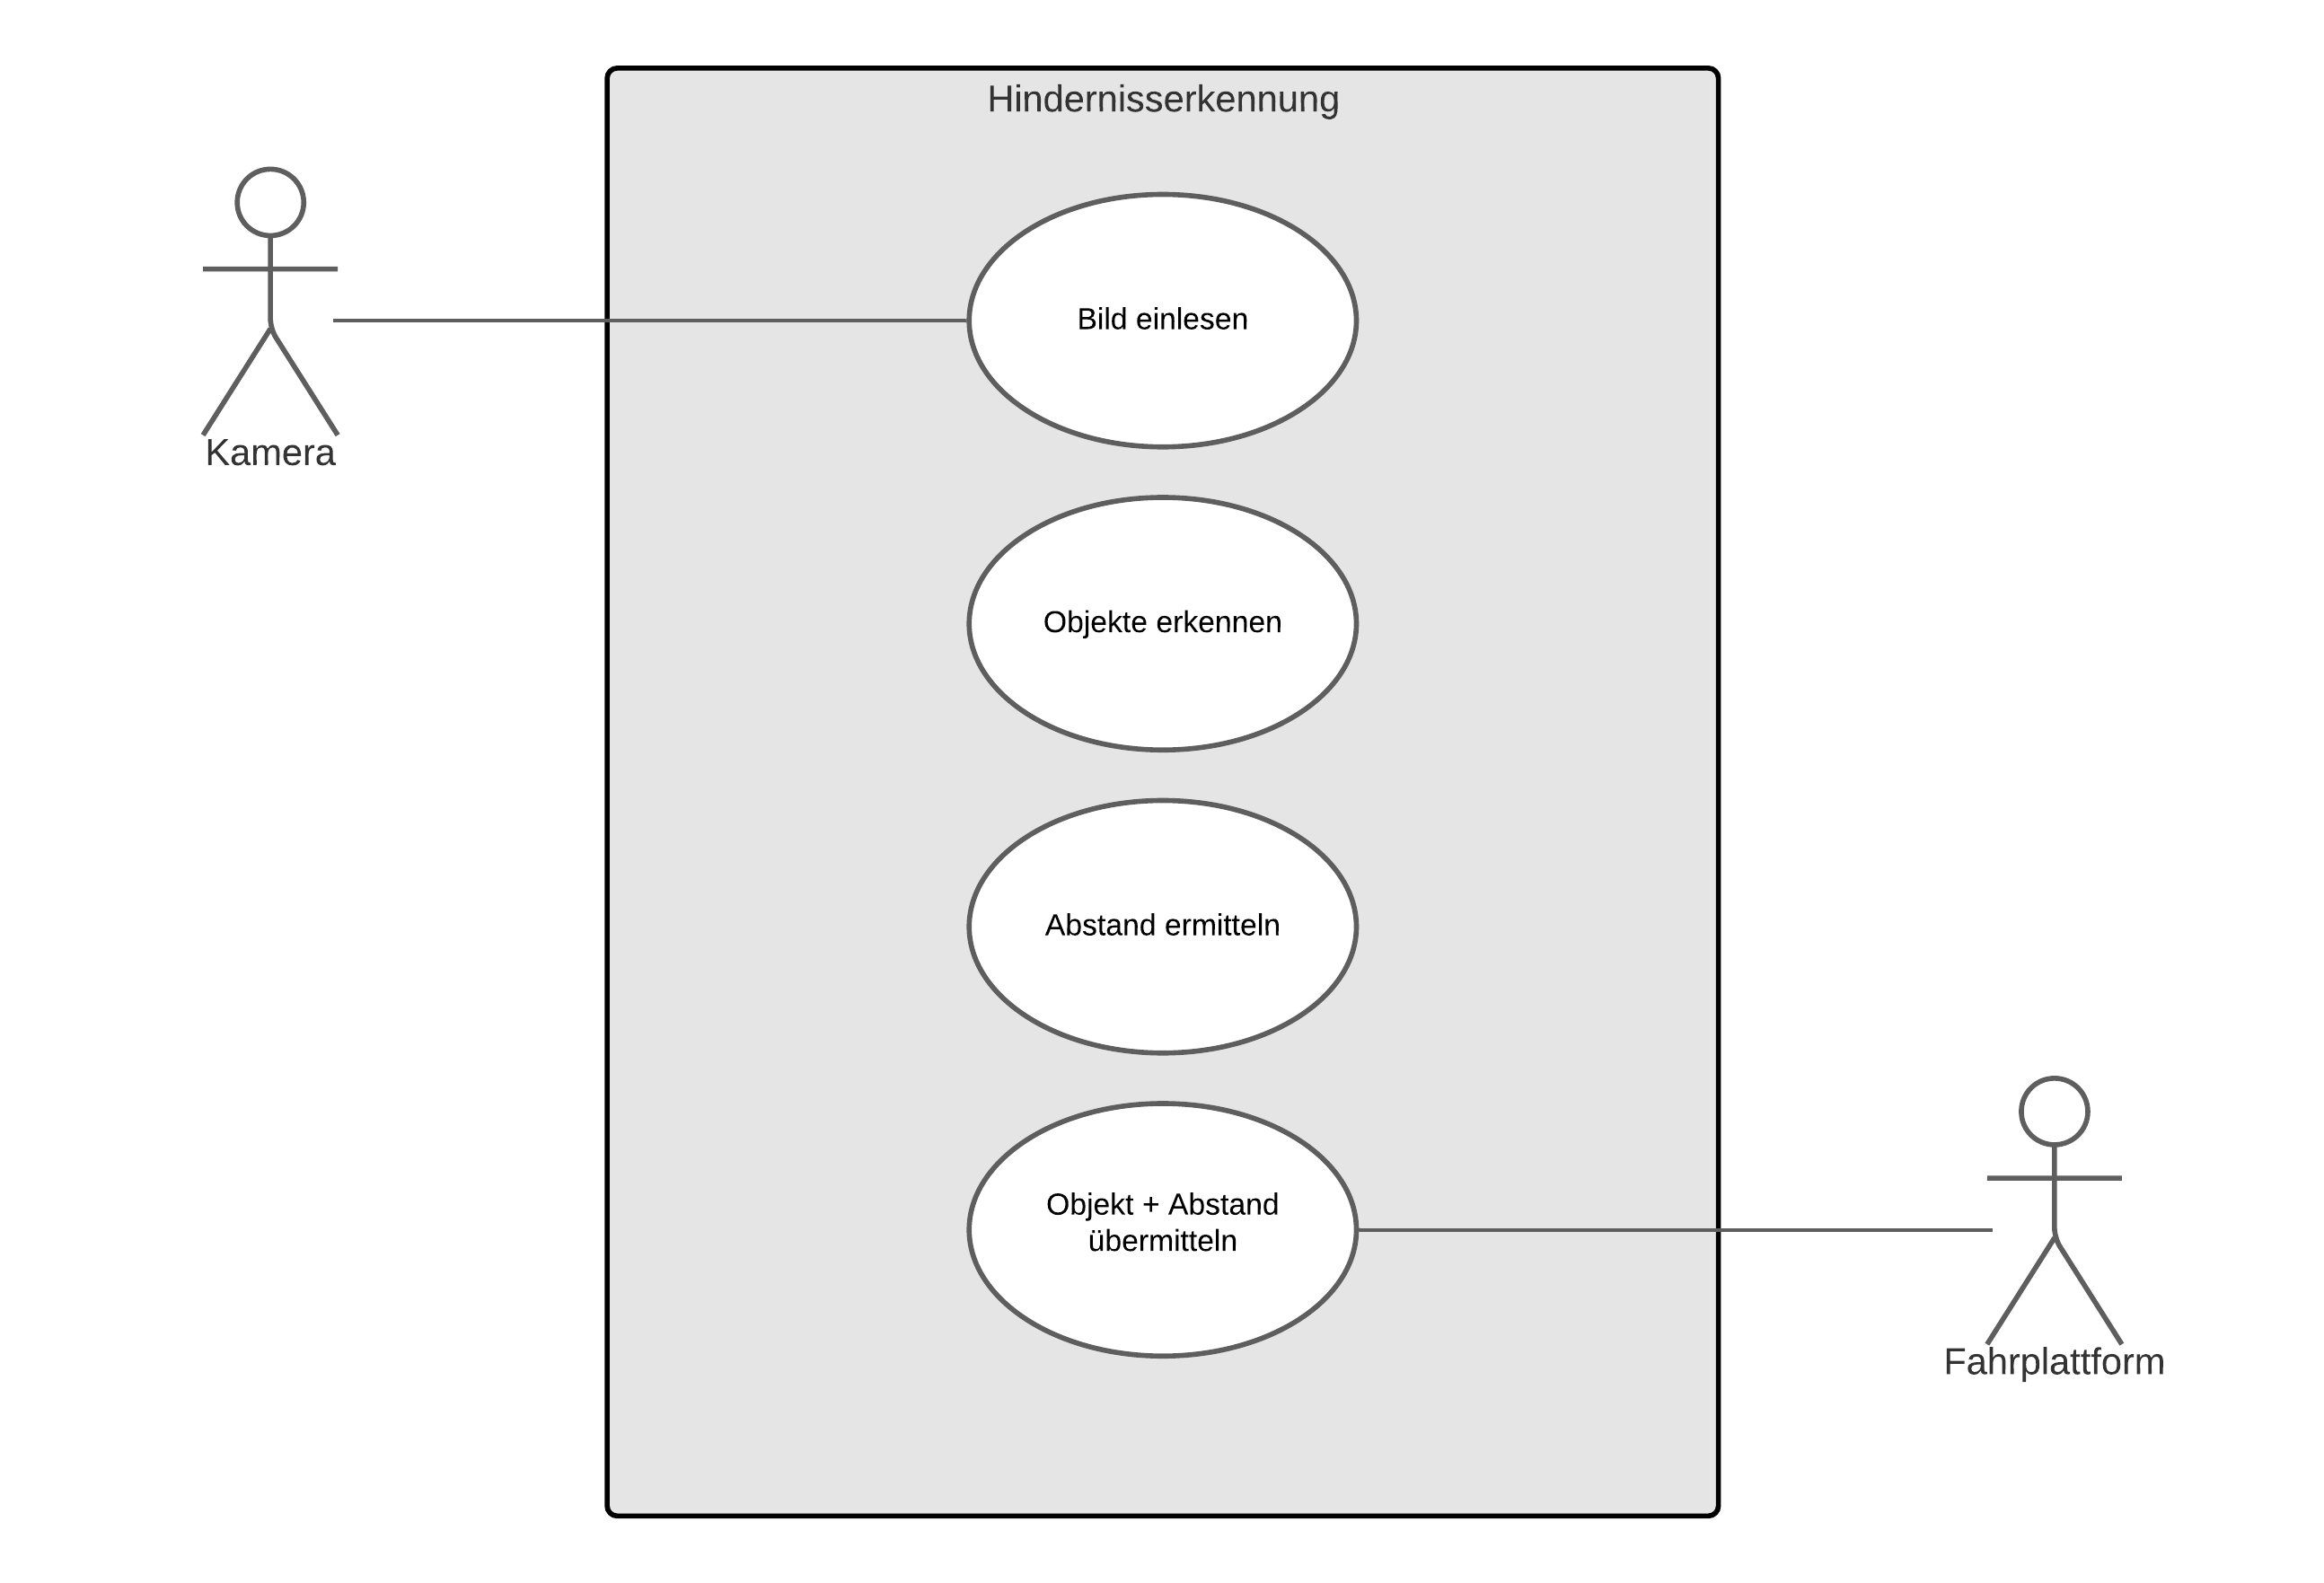
\includegraphics[width=0.9\textwidth]{chapters/cheatsheet/images/UseCaseNeu.png}
		\caption[Box mit höchster $p_{c}$ ist möglicherweise nicht der beste Treffer - Bildquelle: \cite{quickintro}]{Box mit höchster $p_{c}$\\ ist möglicherweise\\ nicht der beste Treffer \cite{quickintro}}
		\label{fig:rasteryolo1a}
	\end{subfigure}%
	\begin{subfigure}[t]{0.35\textwidth}
		\centering
		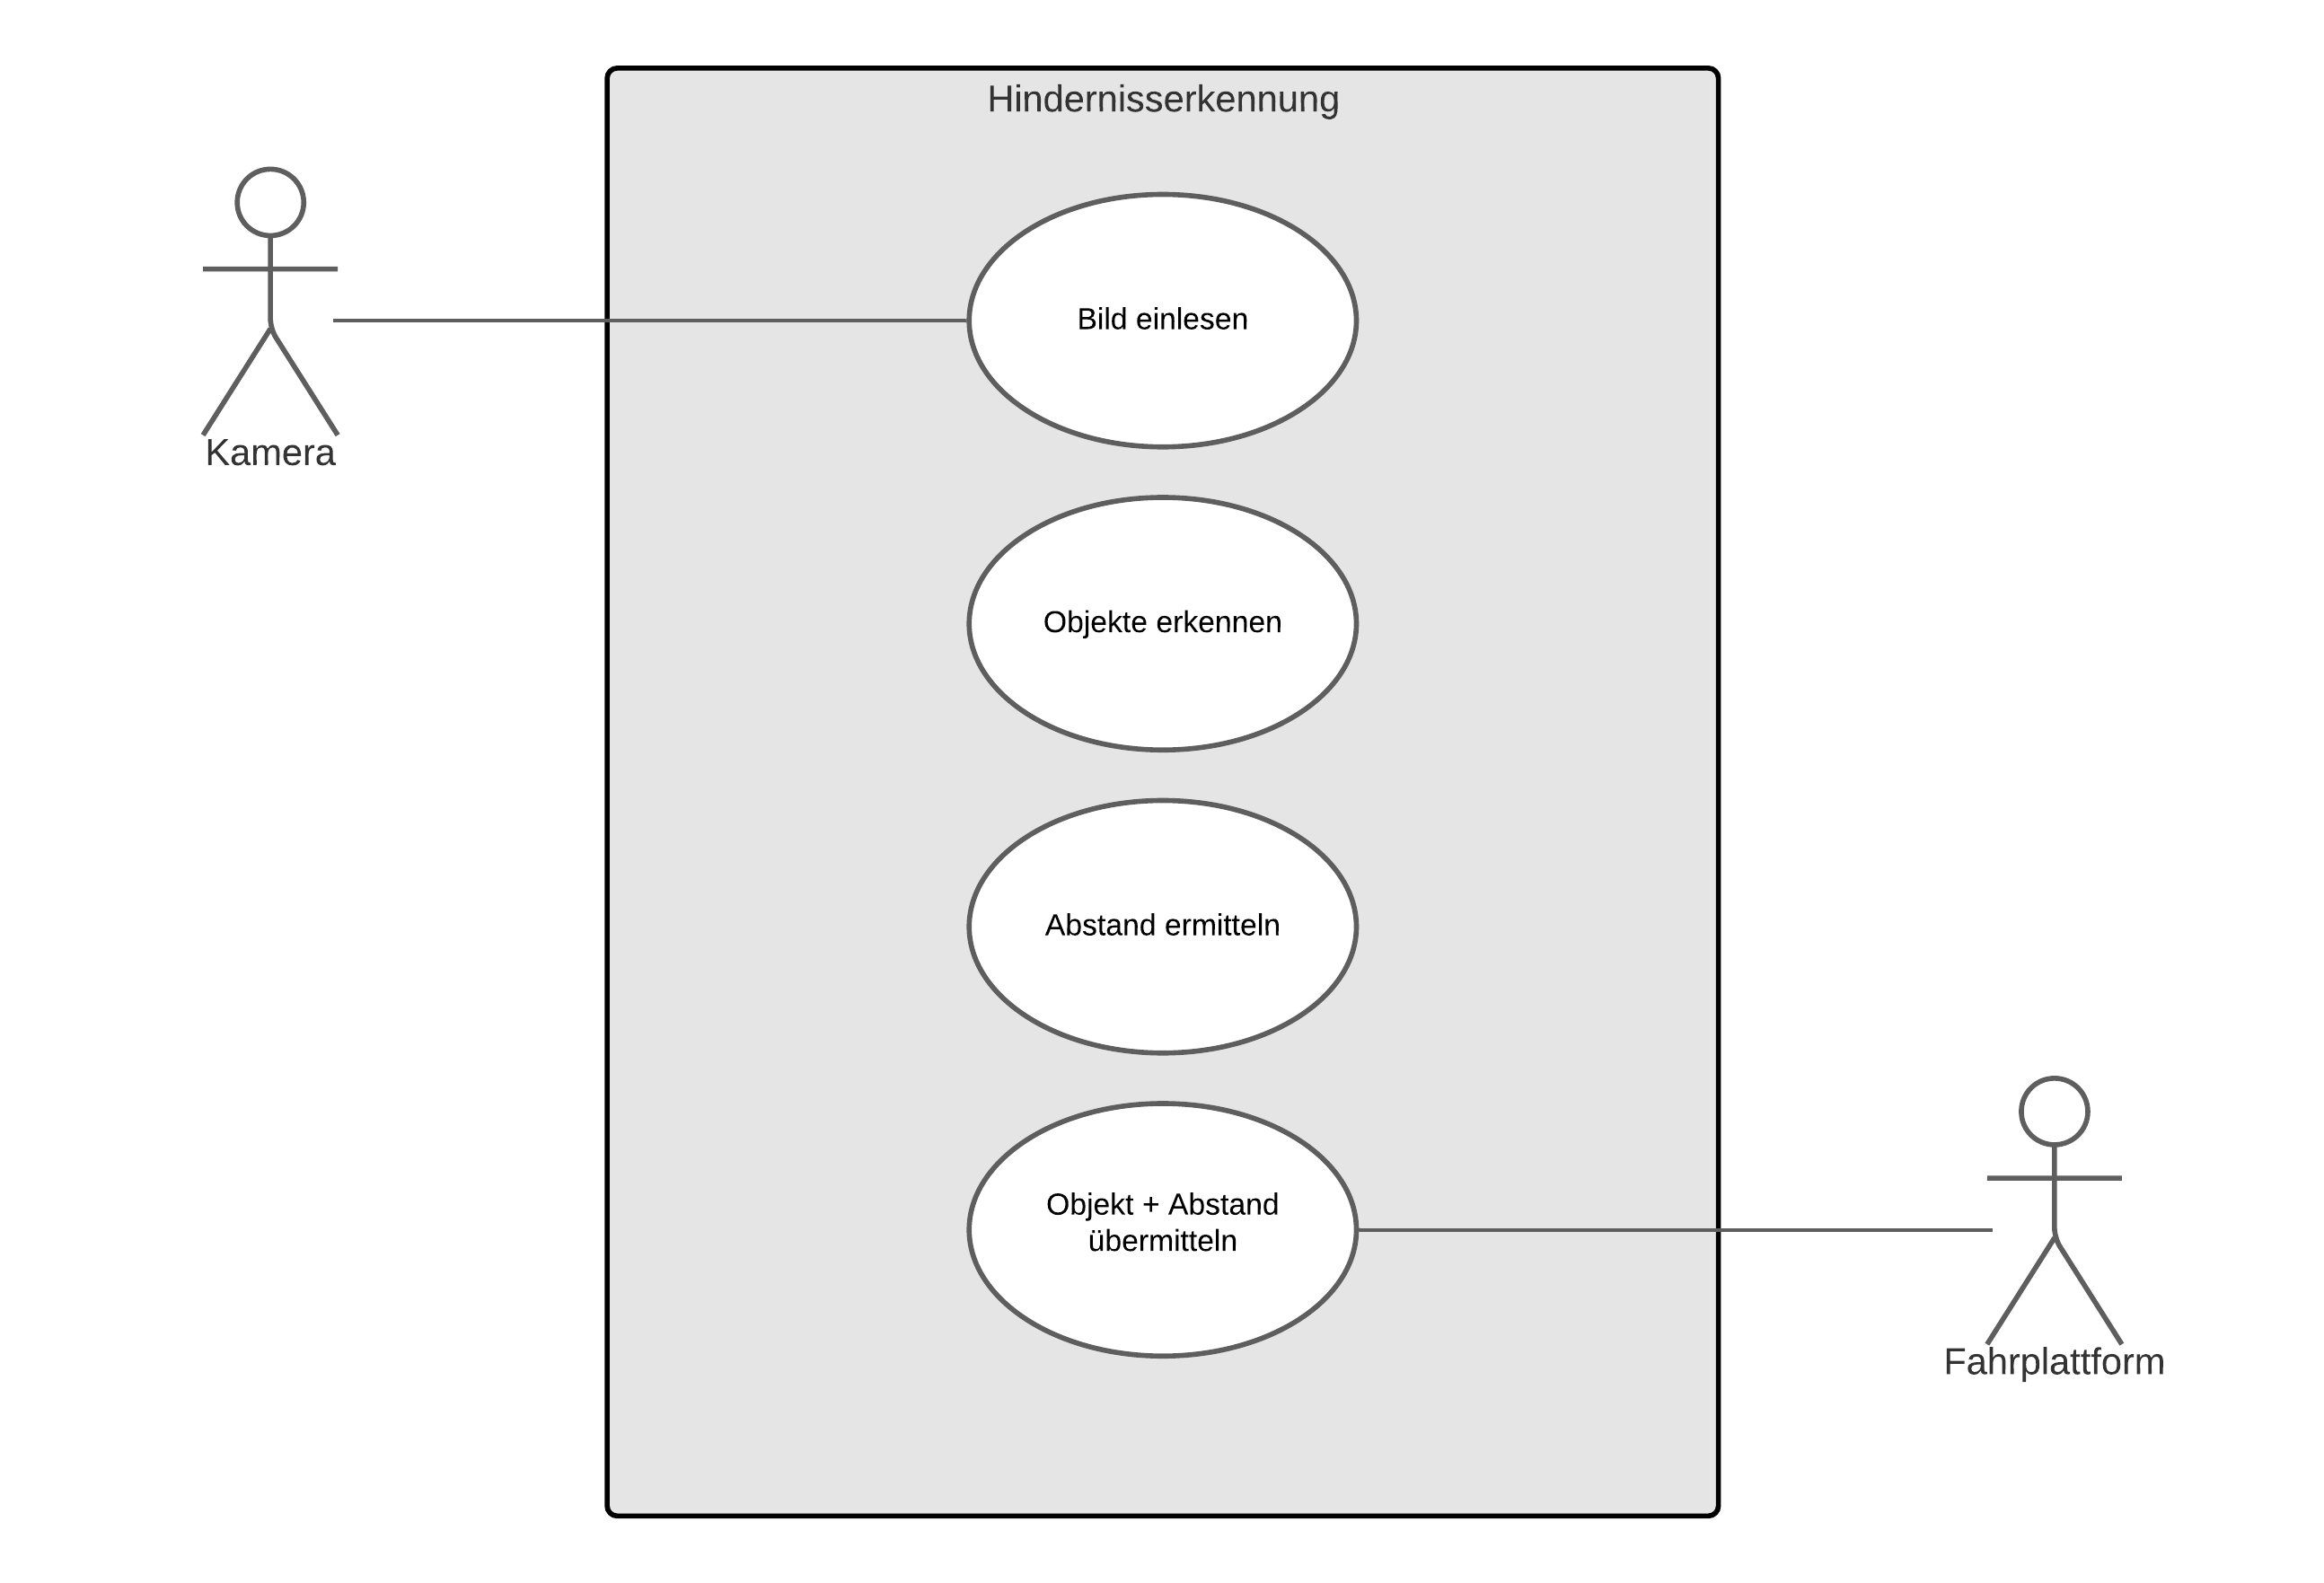
\includegraphics[width=0.8\textwidth]{chapters/cheatsheet/images/UseCaseNeu.png}
		\caption[Kann Objekte in der Nähe verwerfen - Bildquelle: \cite{quickintro}]{Kann Objekte in der\\ Nähe verwerfen \cite{quickintro}}
		\label{fig:rasteryolo1b}
	\end{subfigure}%
	\begin{subfigure}[t]{0.35\textwidth}
		\centering
		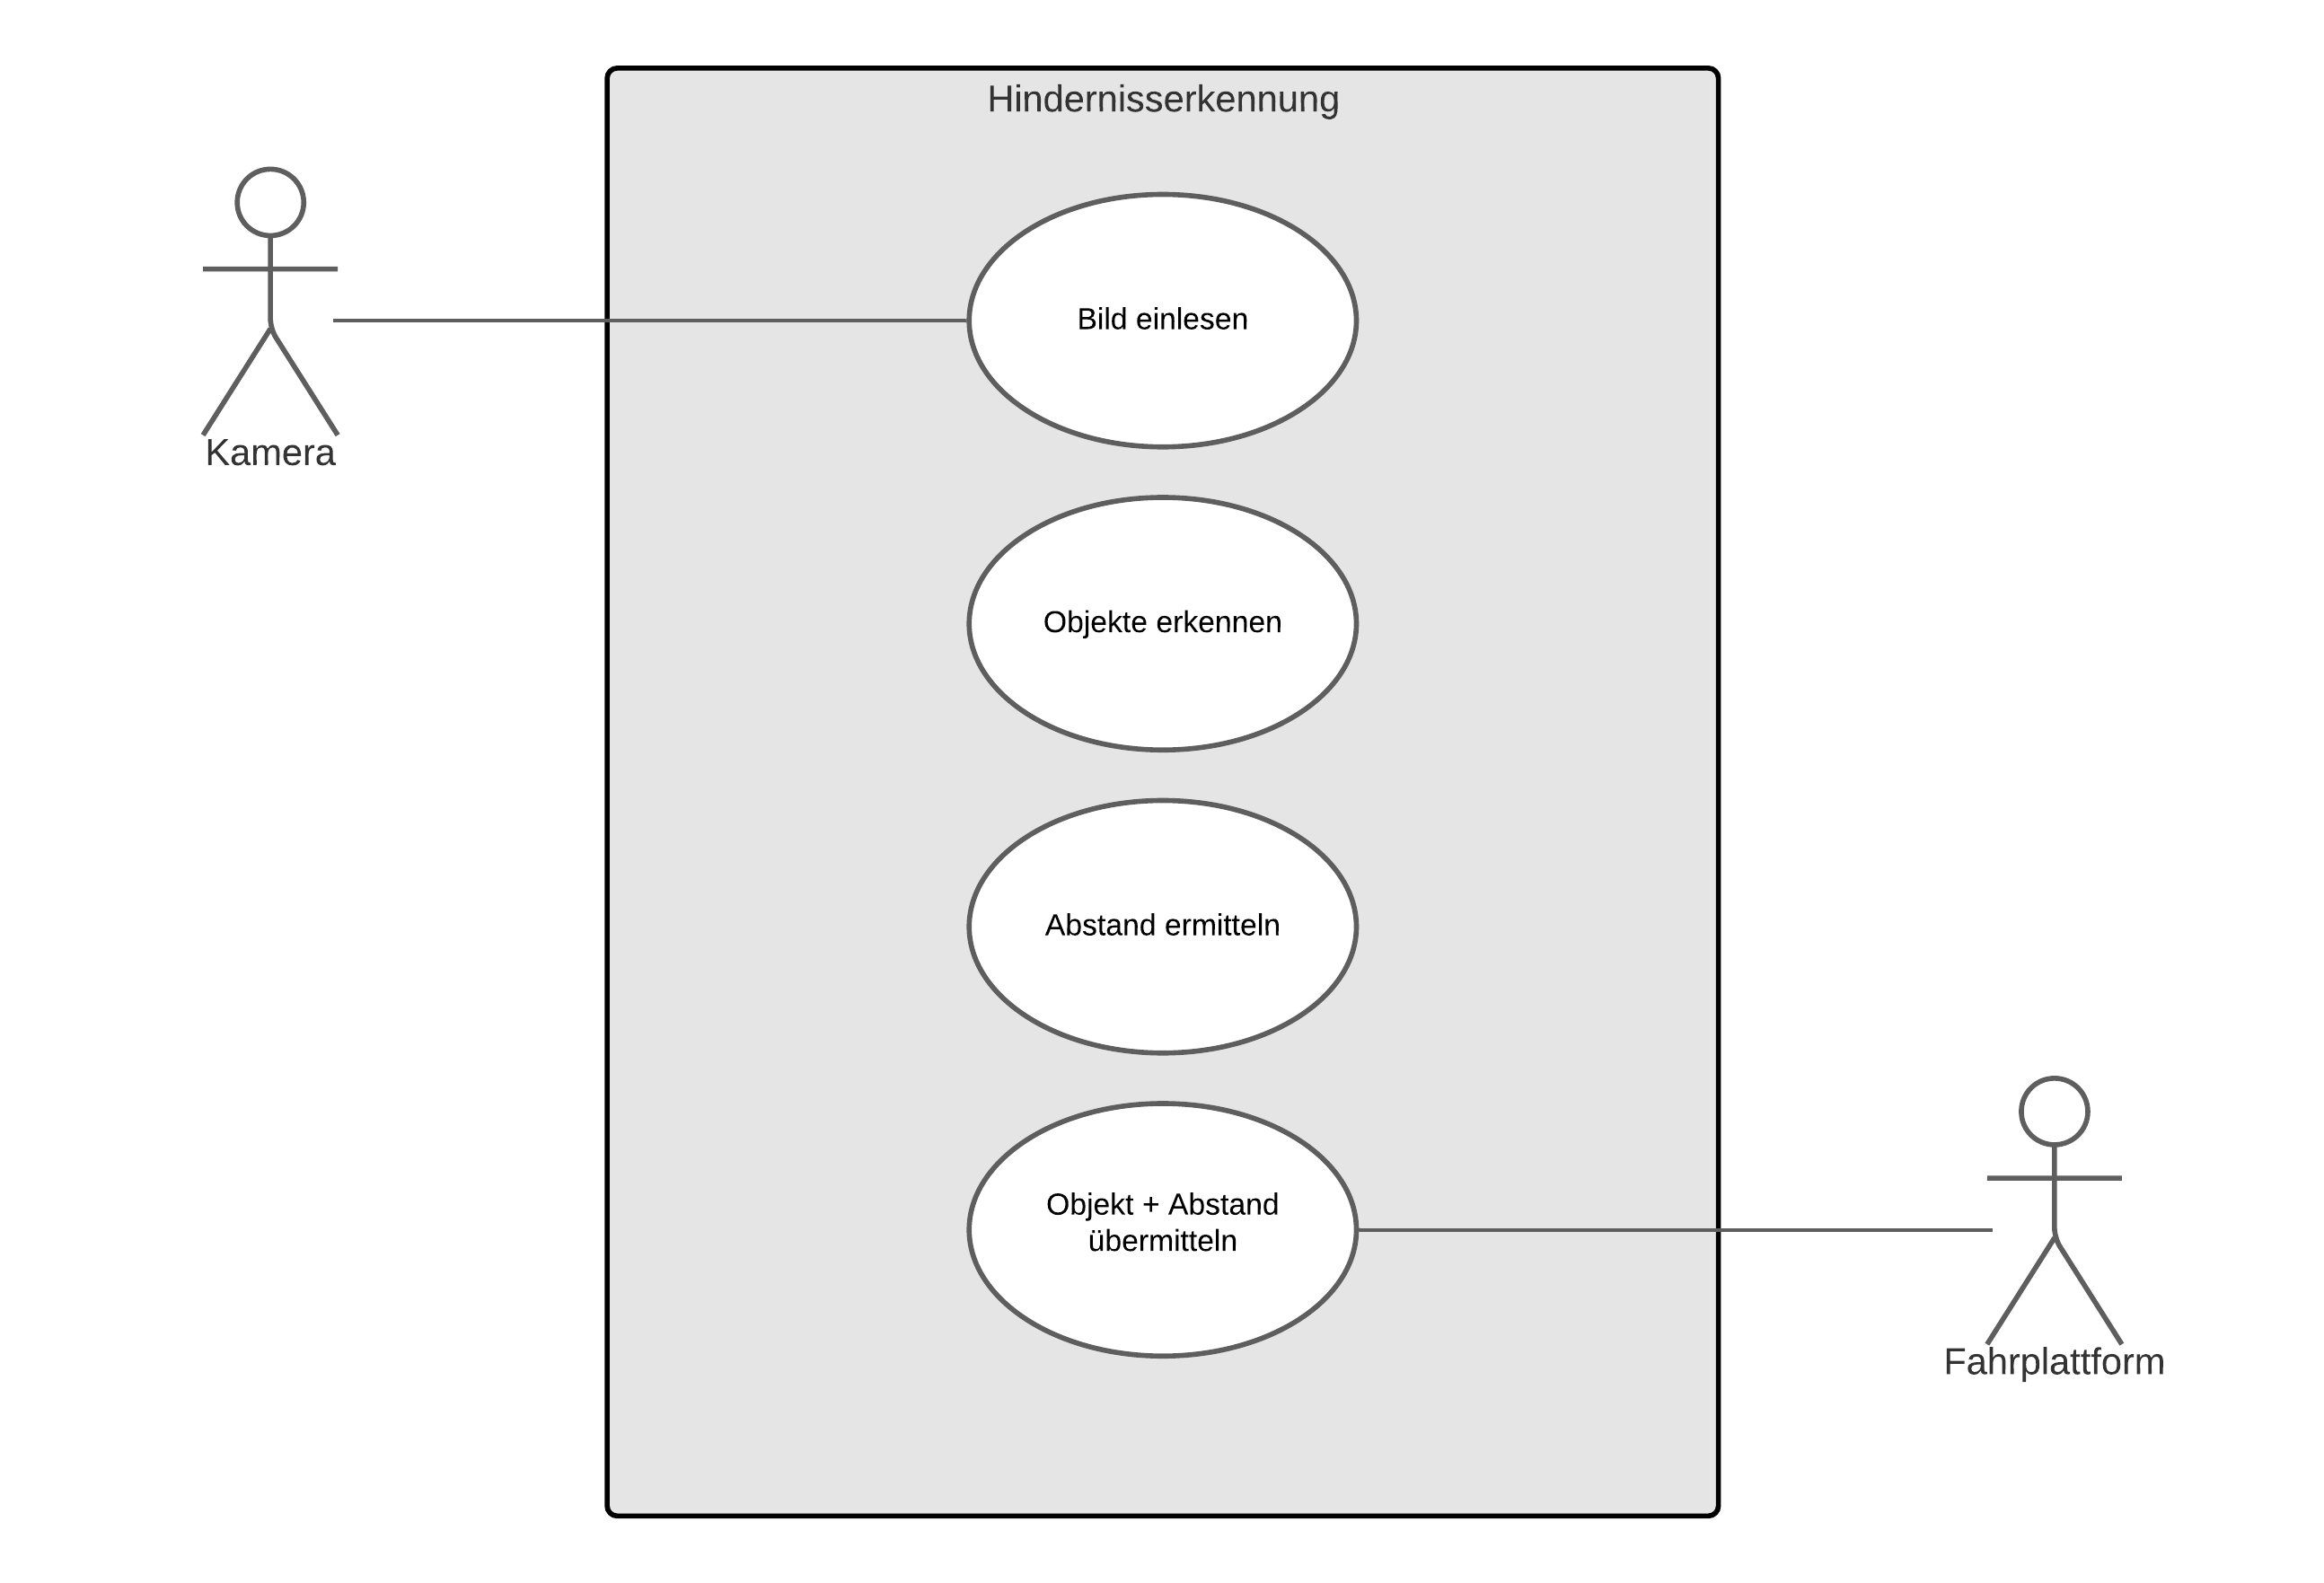
\includegraphics[width=0.9\textwidth]{chapters/cheatsheet/images/UseCaseNeu.png}
		\caption[Verwirft keine False-Positives - Bildquelle: \cite{quickintro}]{Verwirft keine\\ False-Positives \cite{quickintro}}
		\label{fig:rasteryolo1c}
	\end{subfigure}%
	\caption[Problemsituationen NMS - Bildquelle: \cite{quickintro}]{Probleme NMS}
\end{figure}


\begin{minipage}[h]{0.5\textwidth}
	\textbf{YOLO}\\
	Im YOLO-Format wird eine Bounding-Box durch vier Werte [x\_center, y\_center, width, height] dargestellt. Dabei sind x\_center und y\_center die normalisierten Koordinaten des Mittelpunkts der Bounding Box. Um die Koordinaten zu normalisieren, werden die Pixelwerte von x und y durch die Bildbreite x\_max beizehungsweise die Höhe y\_max geteilt.
	\vspace{1mm}
	
\end{minipage}
\begin{minipage}[h]{0.5\textwidth}
	
	\begin{figure}[H]
		\centering
		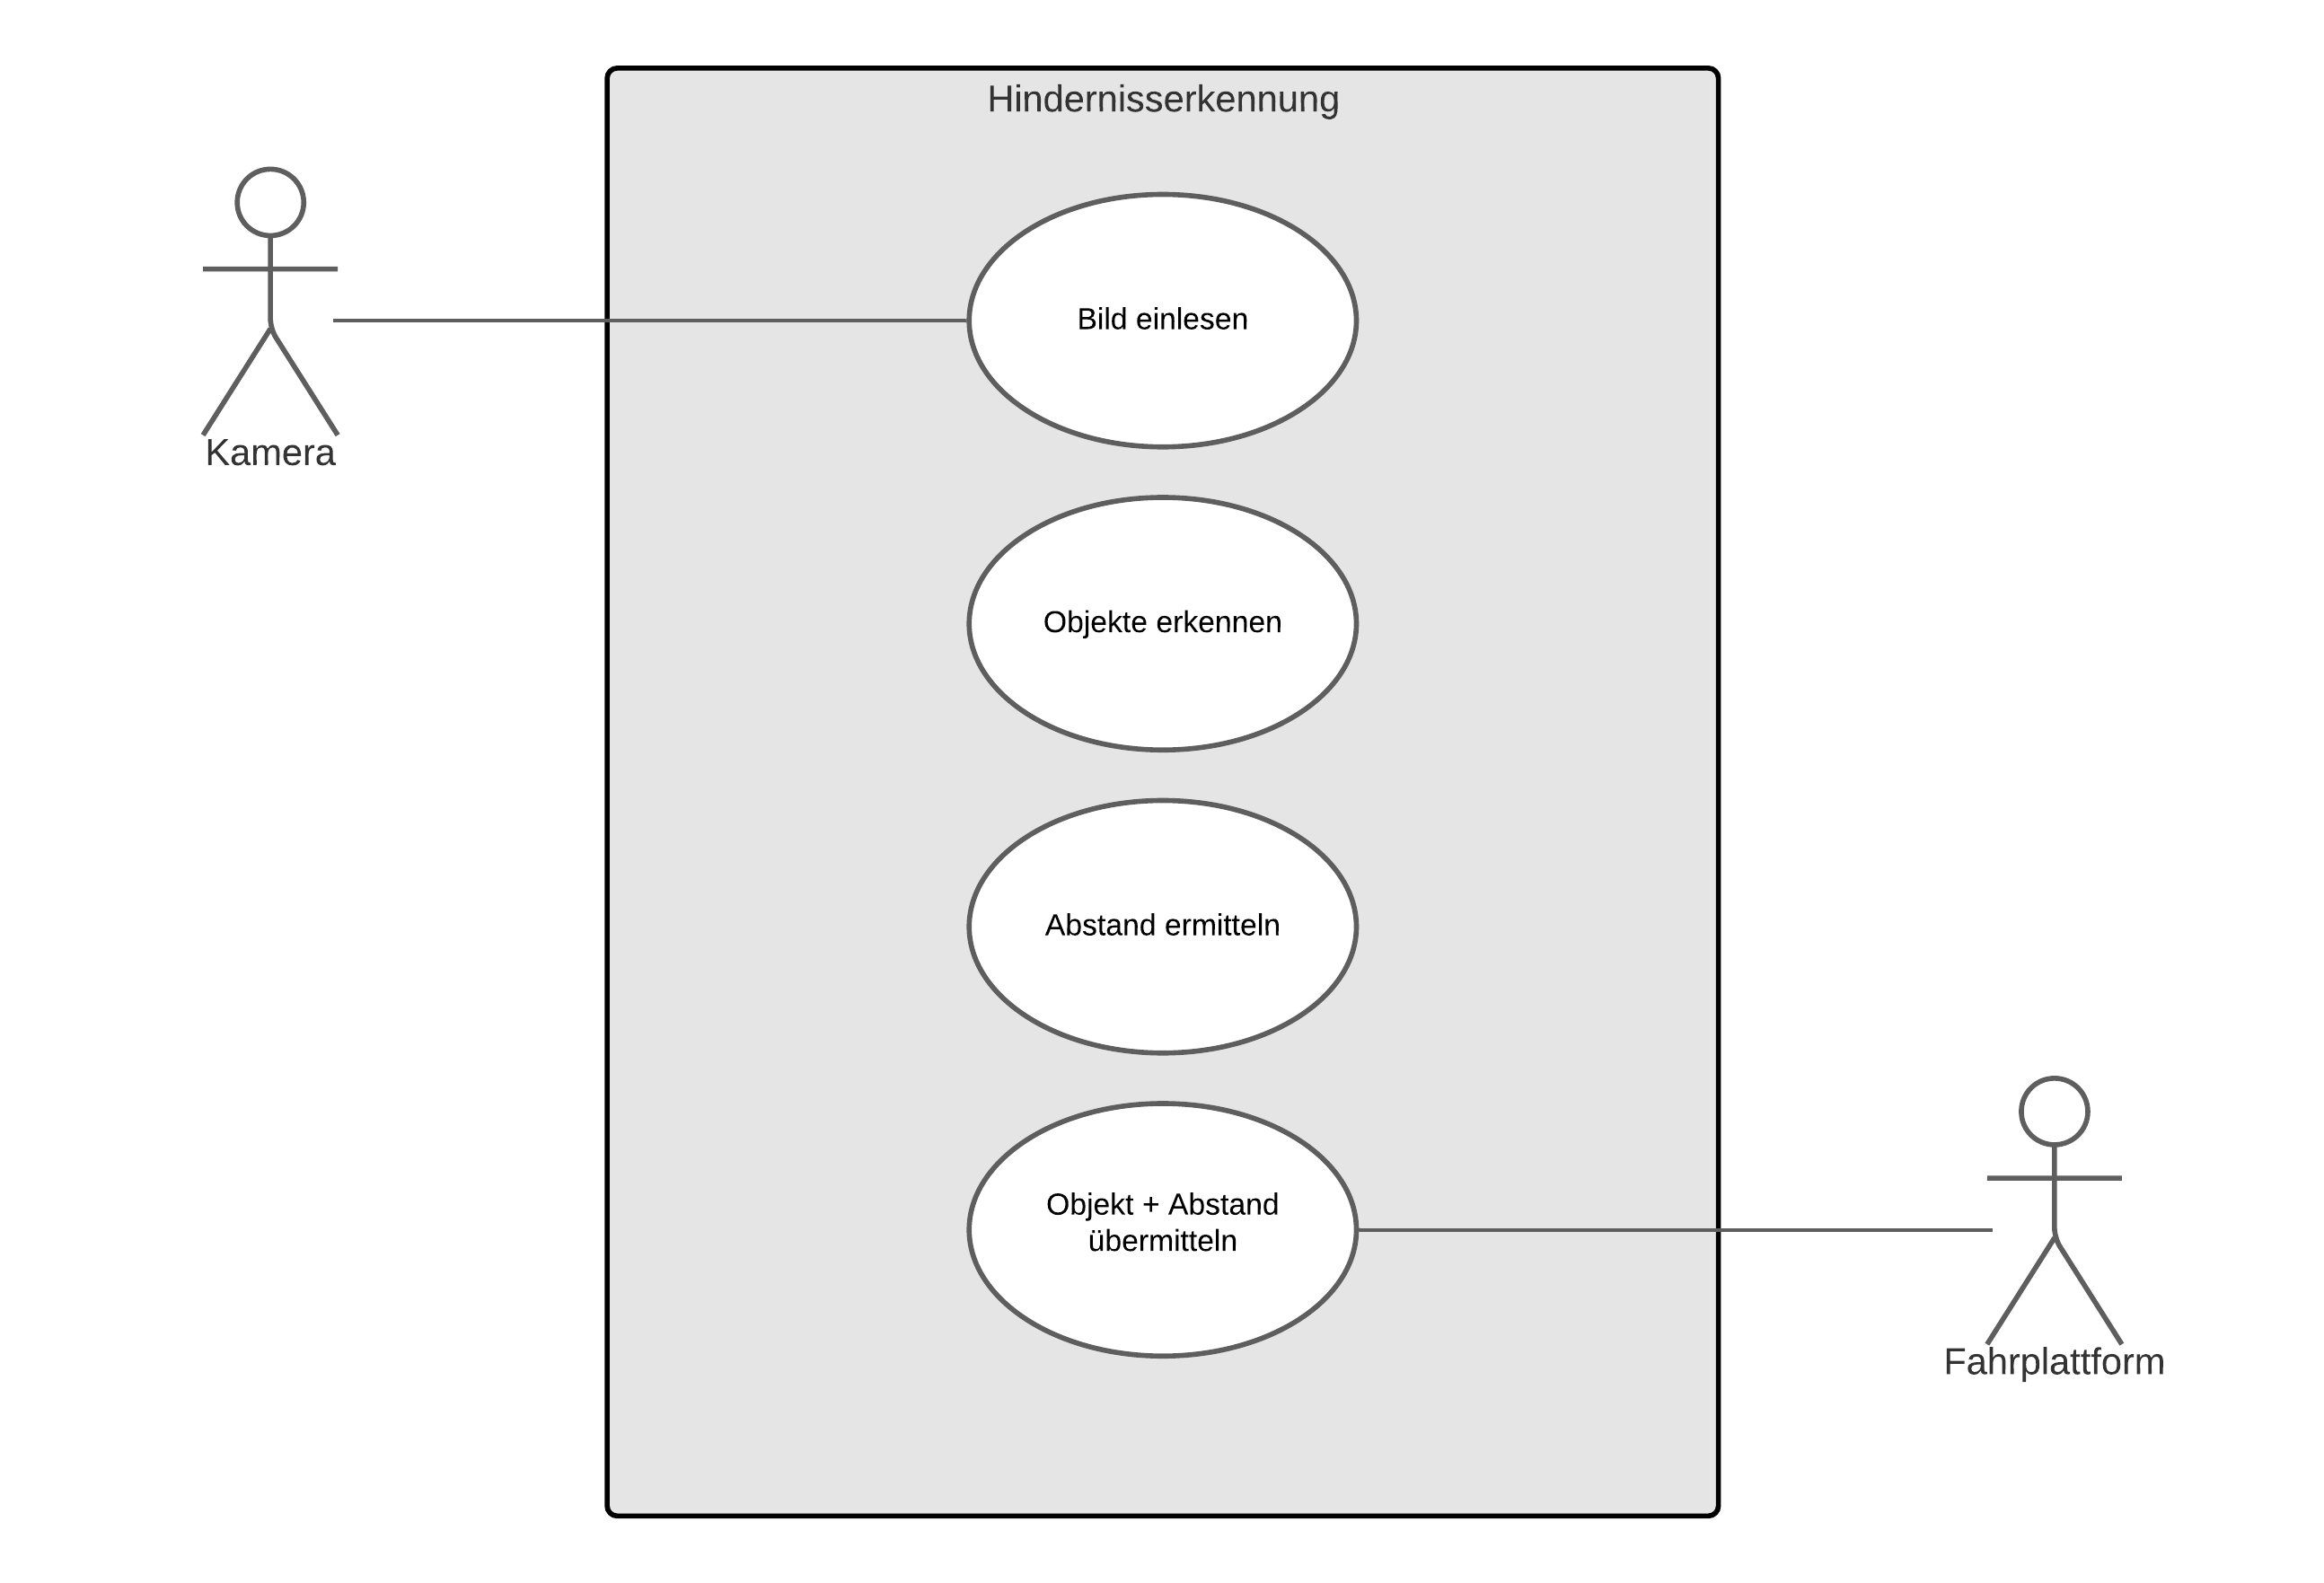
\includegraphics[width=1\textwidth]{chapters/cheatsheet/images/UseCaseNeu.png}
		\caption[Format YOLO - Eigene Darstellung]{Format YOLO}
		\label{fig:format2}
	\end{figure}
	\vspace{1mm}
\end{minipage}
\vspace{1mm}

\section{Formulas}

\begin{minipage}{.5\textwidth}
	\begin{equation}
		\mathbf{g(x, y)}_{x}=\left[\begin{array}{lll}+1 & 0 & -1 \\ +2 & 0 & -2 \\ +1 & 0 & -1\end{array}\right] * \mathbf{f(x, y)}
		\label{eq:sobel1}
	\end{equation}
\end{minipage}%
\begin{minipage}{0.5\textwidth}
	\begin{equation}
		\mathbf{g(x, y)}_{y}=\left[\begin{array}{ccc}+1 & +2 & +1 \\ 0 & 0 & 0 \\ -1 & -2 & -1\end{array}\right] * \mathbf{f(x, y)}
		\label{eq:sobel2}
	\end{equation}
\end{minipage}%




\begin{equation}
	\begin{alignedat}[b]{2}
		& & \zerotext{$\mathrm{~G} =\text{Gegenstandhöhe in Echt in cm}$} \\
		& d=\frac{f \cdot G}{B}& \zerotext{$\mathrm{~B} =\text{Gegenstandhöhe im Bild in Pixel}$} \\
		& & & \zerotext{$\mathrm{~d} =\text {Abstand in cm}$} \\
		& & \zerotext{$\mathrm{~f} =\text {Brennweite in Pixel}$} \\
	\end{alignedat}
\end{equation}




\section{Tables}
\begin{table}[H]
	\centering
	\begin{tabular}[H]{llp{5cm}}
		Augmenter & Parameter & Beschreibung \\ \hline
		& & \\
		Rotate &  $\pm$ 5\textdegree & Bilder werden zufällig bis zu fünf Grad nach links oder rechts um den Bildmittelpunkt gedreht.\\
		& & \\
		Linear Contrast & $\alpha$ = 0.5-1.5  & Erhöht oder verringert Kontrast der Bilder um den Faktor Alpha, der pro Bild zufällig aus einem Intervall gewählt wird.\\
		& & \\
		Motion blur & Kernel = 3x10, horizontal & Den Bildern wird eine horizontale Bewegungsunschärfe hinzugefügt.\\
		& & \\
		Flip & 50\%, horizontal & Bild wird mit einer Wahrscheinlichkeit von 50\% horizontal gespiegelt.\\
		
	\end{tabular}
	\caption{Funktionen der Augmentationspipeline}
	\label{tab:imgaugmenters}
\end{table}


\begin{table}[H]
	\centering	\begin{tabularx}{\textwidth}{|X|c|c|c|}
		\hline
		Phase:  & Median & Mittelwert & Standardabweichung \\ \hline
		Preprocessing: &  - &  - & - \\ \hline
		Inference: &  211 ms & 212 ms & 6 ms \\ \hline
		Postprocessing: &  19 ms & 35 ms & 158 ms \\ \hline
		Gesamt: & 230 ms & 247 ms & 158.11 ms \\ \hline
	\end{tabularx}
	\caption{Performancemessung YoloV5s Pytorch, Auflösung 640x640}
	\label{tab:performYoloV5PT_640}
\end{table}


\section{Code}

\begin{lstlisting}[caption=Training starten]
	%cd /home/$user/yolov5
	!python train.py --img 640 --batch 20 --epochs 600
	--data '../streetsigns.yaml'
	--cfg ./models/yolov5s.yaml
	--weights 'yolov5s.pt'
	--name yolov5s_streetsigns150521_results  --cache
\end{lstlisting}

